% !TEX root = pfe-book2.tex
%!TEX TS-program = pdflatex
%!TEX encoding = UTF-8 Unicode


\cleardoublepage
%\mainmatter
\chapter{Structure of Matter}
\label{ch-02}

\section{Intramolecular Bonds}
Molecules consist of atoms. Atoms are bound in mol­ecules by forces which are called chemical forces.

There exist molecules consisting of two, three, four atoms. The largest molecules, protein molecules, consist of tens and even hundreds of thousands of atoms.

The molecule kingdom is exceptionally varied. By now, millions of substances built up out of various molecules have already been isolated by chemists from natural materials and created in their laboratories.

Properties of molecules are determined not only by how many atoms of one or another sort participate in their construction but also by the order and configura­tion in which they are bound. A molecule is not a heap of bricks, but a complicated architectural structure, where each brick has its place and its completely de­termined neighbours. The atomic structure forming a molecule can be rigid to a greater or lesser degree. In any case, each of the atoms carries out an oscillation about its equilibrium position. In certain cases, some parts of a molecule can even revolve around other parts giving different and the most fantastic configurations to free molecule in the process of its thermal motion.

Let us analyze the interaction between atoms in greater detail. The potential energy curve of a diatomic mole­cule is depicted in \figr{fig-2.1}. It has characteristic form -- it first goes down, then turns up forming a ``well'', and afterwards rises more slowly towards the horizontal axis on which the distance between the atoms is marked.

\begin{figure}[!ht]
\centering
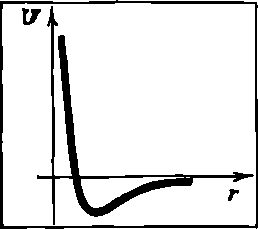
\includegraphics[width=0.4\textwidth]{figures/fig-02-01.pdf}
\caption{The characteristic form of potential energy curve, a potential ``well'' for a diatomic molecule.}
\label{fig-2.1}
\end{figure}

We know that the state in which the potential energy has the minimum value is stable. When an atom forms a part of molecule, it ``sits'' in potential well, carrying out small thermal oscillations about its equilibrium position.

The distance from the vertical axis to the bottom of the well can be called the equilibrium distance. The atoms would be located at this distance if the thermal motion were to cease.

The potential energy curve tells about all the details of the interaction between atoms. Whether particles attract or repel each other at one or another distance, whether the strength of the interaction increases or decreases when the particles separate or approach all this information can be obtained from the analysis of the potential energy curve. Points to the left of the ``bot­tom'' of the well correspond to repulsion. On the contrary, points to the right of the bottom of the well characterize attraction. The steepness of the curve also yields important information: the steeper the curve, the greater the force.

When atoms are at great distances from each other, they are attracted; this force decreases rather rapidly with an increase in the distance -- between them. As they approach each other, the force of attraction grows and readies its maximum value when the atoms come very close to each other. As they come even closer, the attraction weakens and, finally, at the equilibrium distance the force of the interaction vanishes. When the atoms become closer than the equilibrium distance, forces of repulsion arise which sharply increase and quickly make a further decrease in the distance between the atoms practically impossible.

Equilibrium distances (below we shall say distances for the sake of brevity) between atoms are different for various types of atoms.

For various pairs of atoms, not only are the distances between the vertical axis and the bottom of the well different but so are the depths of the wells.

The depth of well has a simple meaning: in order to roll out of the well, an energy just equal to the depth is needed. Therefore, the depth of a well can be called the binding energy of the particles.

The distances between the atoms of molecule are so small that it is necessary to choose appropriate units for their measurement; otherwise, their values would have to be expressed, for example, in the following form: \SI{0.000000012}{\centi\meter}. This figure is for an oxygen molecule.

Units especially convenient for describing the atomic world are called angstroms (true, the name of the Swedish scientist in whose honour these units were named is properly spelt \AA ngstrom; in order to remember this, a small circle is placed over the letter A);
\begin{equation*}%
\SI{1}{\angstrom} = \SI{d-8}{\centi\meter}
\end{equation*}
\SI{1}{\angstrom} is one-hundred-millionth of a centimetre.

The distances between the atoms of a molecule lie within the limits of 1 to \SIrange{1}{4}{\angstrom} The equilibrium distance for oxygen, which has been written out above, is equal to \SI{1.2}{\angstrom}.

Interatomic distances, as you see, are very small. If we gird the Earth with a string at the equator, then the length of the ``belt'' will be as many times greater than the width of your palm as the latter is greater than the distance between the atoms of a molecule.

Ordinary calories are used for measuring binding energies, but they are related not to one molecule, which would, of course, yield a negligible number, but to one mole, i.e. to the number of grams equal to the relative molecular mass.

It is clear that the binding energy per mole divided by Avogadro’s number, $N_{A} = \SI{6.023d23}{\per\mole}$ yields the binding energy of a single molecule.

The binding energy of the atoms in a molecule, just as interatomic distances, varies within narrow limits. For the same oxygen, the binding energy is equal to
\SI{116 000}{\calorie\per\mole}, for hydrogen \SI{103000}{\calorie\per\mole}, etc. We have already said that the atoms in a molecule are distributed in an entirely definite manner with respect to each other, forming in complicated cases rather intricate structures.

Let us present several simple examples. In a molecule
of \ce{CO2} (carbon dioxide), all three atoms are lined up in a row, with the carbon atom in the middle. A molecule of \ce{H2O} (water) has an angular form, with the oxygen atom at the vertex of the angle (it is equal to \ang{105}).

In a molecule of \ce{NH3} (ammonia), the nitrogen atom
is at the vertex of a three-faced pyramid, in a molecule of \ce{CH4} (methane), the carbon atom is located at the centre of a four-faced figure with equal sides, which is called a tetrahedron.

The carbon atoms of \ce{C6H6} (benzene) form a regular hexagon. The bonds of the carbon atoms with the hydro­gen atoms go from all the vertices of the hexagon. All the atoms are situated in one plane.

\begin{figure}[!ht]
\centering
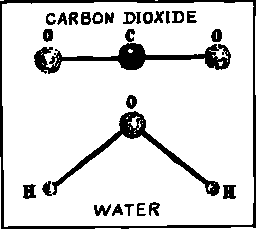
\includegraphics[width=0.4\textwidth]{figures/fig-02-02.pdf}
\caption{Structural form and distribution of atoms in carbon dioxide \ce{CO2} and water \ce{H2O}.}
\label{fig-2.2}
\end{figure}

Diagrams of the distribution of the centres of the atoms in these molecules are shown in \figr{fig-2.2} and \ref{fig-2.3}. The lines symbolize the bonds.

\begin{figure}[!ht]
\centering
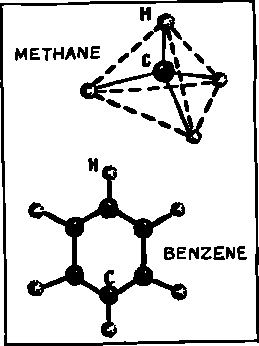
\includegraphics[width=0.4\textwidth,angle=-1]{figures/fig-02-03.pdf}
\caption{Structural form and distribution of atoms in methane \ce{CH4} and benzene \ce{C6H6}.}
\label{fig-2.3}
\end{figure}

A chemical reaction occurred; there were molecules of one type, and then other, were formed. Some bonds were broken, while others, were newly created. In order to break the bonds between atoms (recall \figr{fig-2.1}) it is necessary to perform work, just as in rolling a ball out of a well. On the contrary, energy is liberated when new bonds are formed, just as when a ball rolls into a well.

Which is greater, the work involved in breaking or in creating bonds? We come across reactions of both types in nature.

The excess energy is called the \emph{thermal effect}, or more concisely, the \emph{heat of transformation (reaction)}. The heat of reaction is usually a quantity of the order of tens of thousands of calories per mole. The heat of reac­tion is often included as a summand in the formula for a reaction.
For example, the reaction whereby carbon in the form of graphite burns, i.e. unites with oxygen, is written out as follows:
\begin{equation*}%
\ce{C + O2 -> CO2 + \SI{94250}{\calorie}}
\end{equation*}
This means that when carbon combines with oxygen an energy of \num{94250} calories is liberated.

The sum of the internal energies of a mole of carbon and a mole of oxygen is equal to the internal energy of a mole of carbon dioxide plus \num{94250} calories.

Thus, such formulas have the transparent meaning of algebraic equalities written in terms of the values of the internal energies.

With the aid of such equations, one can find the heats of reaction for which direct methods of measurement, as a result of one or another cause, are unsuitable. Here is an example: if carbon (graphite) were to combine with hydrogen, the acetylene would be formed:
\begin{equation*}%
\ce{2C + H2 -> C2H2}
\end{equation*}
The reaction does not proceed in this manner. Never­theless, it is possible to find its thermal effect. We write down three known reactions:

\begin{enumerate}
\item the oxidation of carbon
\begin{equation*}%
\ce{2C + 2O2 -> 2CO2 + \SI{188000}{\calorie}}
\end{equation*}
\item the oxidation of hydrogen 
\begin{equation*}%
\ce{H2 + 1/2O2 -> H2O + \SI{68000}{\calorie}}
\end{equation*}
\item the oxidation of acetylene 
\begin{equation*}%
\ce{C2H2 + 5/2O2 -> 2CO2 + H2O + \SI{312000}{\calorie}}
\end{equation*}
\end{enumerate}

All these equalities may be regarded as equations for the binding energies of molecules. If so, we may operate on them as on algebraic equalities. Subtracting the first two equalities from the third, we obtain:
\begin{equation*}%
\ce{2C + H2 -> C2H2 - \SI{56000}{\calorie}}
\end{equation*}

Therefore, the reaction we are interested in is accom­ panied by the consumption of \num{56000} calories per mole.

\section{Physical and Chemical Molecules}

Until investigators had formed a detailed concept of the structure of matter, no such distinction was made. A molecule was simply a molecule, i.e. the smallest representative of a substance. It seemed that nothing more could be said. This is not so, however.

The molecules we have just discussed are molecules in both senses of the word. Molecules of carbon dioxide, ammonia and benzene (mentioned above), and the mol­ecules of practically all organic substances (which were not discussed) consist of atoms strongly bonded to one another. These bonds are not ruptured by dissolution, melting or evaporation. The molecule continues to be­ have as a separate particle or small physical body upon any physical action or change in state.

But this is not always true. For most inorganic sub­stances, we can speak of the molecule only in the chem­ical sense. The finest particles of such well-known inorganic substances as common salt or calcite or soda do not even exist. We do not find separate particles of these substances in crystals (this will be discussed a few pages further on); when they are dissolved, the molecules break down into their component atoms.

Sugar is an organic substance. Therefore, the sugar dispersed in a cup of sweetened tea is in the form of molecules. Salt is a different matter. We find no molecules of common salt (sodium chloride) in salty water. These ``molecules'' (we have to use quotation marks) exist in water in the form of atoms (actually, ions -- electrically charged atom -- that will be discussed later).

The same is true of vapours; and in melts a part of, the molecules live their own independent lives. 

When we speak of the forces binding the atoms together in a physical molecule, we call them valence forces. Intermolecular forces are not of the valency kind. The general shape of the interaction curve, of the type il­lustrated in \figr{fig-2.1}, is the same for both kinds of forces. The difference lies in the depth of the potential well. For valence forces the well is hundreds of times deeper.


\section{Interaction of Molecules}
There can be no doubt of the fact that molecules at­tract each other. If they stopped doing so for an instant, all liquids and solids would decompose into molecules.

Molecules repel each other, and neither can this be doubted, because liquids and solids would otherwise contract with extraordinary ease.
Forces are exerted between molecules which resemble in many respects the forces between atoms spoken of above. The potential energy curve which we have just drawn for atoms gives a true picture of the basic features of molecular interaction. However, there are also es­sential differences between these interactions.

Let us compare, for example, the equilibrium distances between oxygen atoms forming a molecule and oxygen atoms of two neighbouring molecules attracted in solidified oxygen before the equilibrium position. The difference will be very noticeable: the oxygen atoms forming a molecule settle down at a distance of \SI{1.2}{\angstrom}, while the oxygen atoms of different molecules approach each other to within \SI{2.9}{\angstrom}.

Analogous results have also been obtained for other atoms. Atoms of different molecules settle down farther from each other than atoms of the same molecule. It is therefore easier to tear molecules apart from each other than atoms from a molecule; moreover, the difference in energy is much greater than that in distance. While the energy necessary for breaking the bonds between oxygen atoms forming a molecule is about \SI{100}{\kilo\calorie\per\mole}, the energy needed to pull oxygen molecules asunder is less than \SI{2}{\kilo\calorie\per\mole}.

Hence, on a potential energy curve for molecules, the potential well lies farther away from the vertical axis and, furthermore, the well is much shallower.

However, this does not exhaust, the, difference between the interaction between atoms forming a molecule and the interaction of molecules.

Chemists have shown, that atoms are bound in a mole­cule with a fully determined number of other atoms. If two hydrogen atoms have formed a molecule, no third atom will join them to this end. A oxygen atom in water is bound to two hydrogen atoms, and it is im­possible to bind another atom to them.

We do not find anything similar in intermolecular interaction. Having attracted one neighbour to itself, a molecule does not lose its ``attractive force'' to any degree. The approach of neighbours will continue, as long as there, is enough room.

What does ``there is enough room'' mean? Are molecules really something, like apples or eggs? Of course, in a certain sense such a comparison is justified: molecules are physical bodies possessing definite size and shape. The equilibrium distance between molecules is nothing but their size.


\section{What Thermal Motion Looks Like}
The interaction between molecules can have greate or smaller values during the ``lives'' of the molecules.

The three states of matter -- gaseous, liquid and solid -- differ from one another in the role which molecular interaction plays in them. The word ``gas'' was thought up by scientists (derived from the Greek \emph{chaos} meaning ``disorder'').

And as a matter of fact, the gaseous state of matter is an example of the existence in nature of complete, perfect disorder in the mutual distribution and motion of particles. There is no microscope which would permit one to see the motion of gaseous molecules, but in spite of this, physicists can describe the life of this invisible world in sufficient detail.

There is an enormous number of molecules, approximate­ly \num{2.5d19} molecules in a cubic centimetre of air under standard conditions (room temperature and atmo­spheric pressure). Each molecule’s share is a volume of \SI{4d-20}{\centi\meter\cubed}, that of a small cube whose sides are approximately $\SI{3.5d-7}{\centi\meter} = \SI{35}{\angstrom}$. However, the molecules are much smaller. For example, molecules of oxygen and nitrogen -- the basic components of air -- have an average size of about \SI{4}{\angstrom}.

Therefore, the average distance between molecules is ten times as great as the size of the molecules. And this in turn implies that the average volume of air per molecule is approximately a thousand times as great as the volume of the molecule itself.

Imagine a plane surface on which coins have been thrown in a random manner where there is an average of a hundred coins to each square metre. This means one or two coins on a page of the book which you are reading. This is roughly how sparsely gas molecules are distrib­uted.

Every molecule of a gas is in a state of continual thermal motion.

Let us follow a single molecule. Here it is swiftly moving somewhere to the right. If it met no obstacles in its path, the molecule would continue its motion with the same velocity along a straight line. But the path of the molecule is crossed by its innumerable neighbours. Collisions are inevitable, and the molecules fly apart like two colliding billiard balls. In which direction will our molecule gallop? Will it acquire or lose its speed? Anything is possible: for its collisions can be of the most various kinds. Blows are possible from the front or from behind, from the right or the left, which are strong or weak. It is clear that being subject to such irregular impacts during these random collisions, the molecule which we are observing will rush about through all parts of the vessel in which gas is confined.

How far are gas molecules able to go without a col­lision?

It depends on the size of the molecules and the density of the gas. The larger the molecules and the more mole­cules there are in a vessel, the more often will they collide. The average distance travelled by a molecule without any impact -- it is called the mean free path -- is equal to $\SI{11d-8}{\centi\meter} = \SI{1100}{\angstrom}$ for hydrogen mole­cules and $\SI{5d-6}{\centi\meter} = \SI{500}{\angstrom}$ for oxygen molecules under ordinary conditions. The distance of \SI{5d-6}{\centi\meter} (one-twenty-thousandth of a millimetre) is very small, but it is far from small in comparison with molecular sizes. A distance of \SI{10}{\meter} for a billiard ball corresponds in scale to a path of \SI{5d-6}{\centi\meter} for an oxygen molecule.

The structure of a liquid differs essentially from that of a gas whose molecules are far from each other and only rarely collide. In a liquid, a molecule is constantly found in the immediate vicinity of others. The molecules of a liquid are distributed like potatoes in a sack. True, with one distinction: the molecules of a liquid are in a state of continual and chaotic thermal motion. Because they are so crowded, they cannot move around as freely as the molecules of a gas. Each of them is always ``marking time'' in practically one and the same place surrounded by the same neighbours, and only gradually moves through the volume occupied by the liquid. The more viscous the liquid, the slower this displacement. But even in such a ``mobile'' liquid as water, a molecule moves \SI{3}{\angstrom} during the time required by a gas molecule to cover \SI{700}{\angstrom}.

The forces of interaction between molecules deal very resolutely with their thermal motion in solids. In solid matter, the molecules are almost always in a fixed posi­tion. The only effect of the thermal motion is that the mole­cules are continually vibrating about their equilibrium positions. The lack of systematic displacements by the molecules is precisely the cause of what we call solidity. In fact, if molecules do not change neighbours, all the more will the separate parts of the body remain in a fixed bond with one-another.

\section{Compressibility of Bodies}

As raindrops drum on a roof, so do gas molecules beat against the walls of a vessel. The number of these blows is immense, and it is their united action that creates the pressure which can move the piston of an engine, explode a shell or blow up a balloon. A hail of molecular blows -- this is atmospheric pressure, this is the pressure that makes the lid of a boiling tea-kettle jump, this is the force driving a bullet out of a rifle.

What is gas pressure related to? It is clear that the
stronger the blow inflicted by a single molecule, the greater the pressure. It is no less obvious that the pressure will depend on the number of blows inflicted in a second. The more molecules in a vessel, the more frequent the blows and the greater the pressure. Hence, the pressure $p$ of a given gas is proportional, first of all, to its density.

If the mass of gas is constant, then decreasing its volume, we increase its density by the corresponding factor. Therefore, the pressure of a gas in a closed vessel will be inversely proportional to its volume. Or, in other words, the product of the pressure by the volume must be constant:
\begin{equation*}%
pV = \textrm{const}
\end{equation*}
This simple law was discovered by the English physi­cist Robert Boyle (1627-1691) and the French scientist Edme Mariotte (c.~1620-1684). \emph{Boyle's law} (also known as \emph{Mariotte's law}) is one of the first quantitative laws in the history of physical science. Of course, it holds when the temperature is constant.

As a gas is compressed, the Boyle equation is satisfied worse, and worse. The molecules approach each other and, the interactions between them begin to influence the, behaviour of the gas.

Boyle’s law is valid in those cases when the inter­ference of the forces of interaction between the gas mole­cules is completely insignificant. One therefore speaks of Boyle’s, law as a law of ideal gases.

The adjective ``ideal'' sounds rather funny when modi­fying the word ``gas''. Ideal means perfect, so that it is impossible to be better. 

The simpler a model or diagram, the more ideal it is for the physicist. Computations are simplified, explana­tions of physical phenomena become easy and clear. The term ``ideal gas'' pertains to the simplest model of a gas. The behaviour of sufficiently rarefied gases is practically indistinguishable from that of ideal gases.

Liquids are much less compressible than gases. In a liquid, the molecules are already in ``contact''. Compres­sion consists only in improving the ``packing'' of the molecules, and for very high pressures, in pressing the molecules themselves. The degree to which the forces of repulsion hinder the compression of a liquid can be seen from the following figures. A rise in pressure from one to two atmospheres entails a decrease in the volume of a gas by a factor of two, while the volume of water changes by 1/\num{20000} and that of mercury by total of 1/\num{250000}.

Even the enormous pressure in the depths of an ocean is incapable of compressing water to any noticeable extent. In fact, a pressure of one atmosphere is created by a ten-metre column of water. The pressure under a \SI{10}{\kilo\meter} layer of water is equal to \SI{1000}{\atmos}. The volume of water decreases by 1000/\num{20000}, i.e. by one-twen­tieth.

The compressibility of solids differs little from that of liquids. This is understandable since in both cases the molecules are already in contact, and so compression can only be achieved at the expense of a further drawing together of molecules which are already strongly repelling each other. By means of ultrahigh pressures of 50-100 thou­sand atmospheres, we are able to compress steel by one-thousandth, and lead by one-seventh, of its volume.

It is clear from these examples that, under terrestrial conditions, we cannot succeed in compressing solid mat­ter to any significant extent.

But in the Universe, there are bodies where matter is compressed with incomparably greater strength. Astron­omers discovered the existence of stars in which the density of matter reaches \SI{d8}{\gram\per\centi\meter\cubed}. Inside these stars, called white dwarfs (``white'' for the nature of their lumi­nosity, ``dwarfs'' because of their relatively small size), there should therefore be enormous pressures.


\section{Surface Tension}

Is it possible to emerge dry from water? Of course it is, if one smears oneself with a non-wettable substance. Rub your finger with paraffin and put it under water.

When you take it out, you will find that except for two or three drops there is no water on your finger. A slight motion -- and the drops are shaken off.

In this case we say that water does not wet paraffin. Mercury behaves in such a manner towards almost all solid bodies: it does not wet leather, glass or wood. 

Water is more capricious. It adheres closely to some bodies and tries not to touch others. Water does not wet oily surfaces, but thoroughly wets clean glass. Water wets wood, paper and wool.

If a drop of water is placed on a clean plate of glass, it will spread out and form a very shallow, small puddle. If such a drop is put on a piece of paraffin, it will just remain a drop, almost spherical in shape and slightly flattened by gravity.

Among the substances which ``stick'' to almost all bodies is kerosene. Striving to flow along glass or metal, kerosene is capable of creeping out of a loosely closed vessel. A puddle of spilled kerosene can spoil one’s existence for a long time: kerosene will seize a large sur­face, creep into cracks and penetrate one’s clothes. That is why it is so difficult to get rid of its not very pleasant odour.

The failure to wet bodies can lead to curious phenomena. Take a needle, grease it and carefully place it flat on water. The needle will not sink. Looking attentively, you can notice that the needle depresses the water and calmly lies in the small hollow so formed. However, a slight pressure is enough to make the needle go to the bottom. For this it is necessary that a considerable part of it turns out to be in the water.



 This interesting property is made use of by water strid­ers running swiftly along the surface of the water with­ out wetting their feet.
 
Wetting is used to dress ores by means of floatation. The word ``floatation'' means ``surfacing''. The essence of the phenomenon is as follows. Finely crushed ore is loaded into a vat containing water. A small amount of special oil is added; this oil must wet the particles of the mineral and not wet the particles of the gangue (this is what the valueless rock or aggregates of minerals in an ore are called). When mixed, the particles of the mineral are coated with an oily film.

Air is blown into the black mixture of ore, water and oil. There is formed a mass of little bubbles of air -- foam. The air bubbles come to the surface. The process of floatation is based on the fact that the particles coated with oil cling to the air bubble. A large bubble drags up a small particle like a balloon.

The mineral collects at the surface in the form of foam and the gangue remains at the bottom. The foam is moved and sent for further processing order to obtain a so-called ``concentrate'', which contains tens of times as little gangue.


Forces of cohesion between surfaces are capable of violating the levelling of a liquid in communicating vessels. It is very easy to verify the truth of this.

\begin{figure}[!ht]
\centering
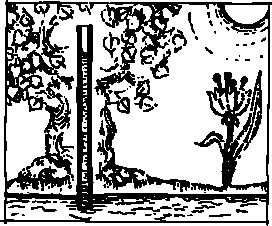
\includegraphics[width=0.6\textwidth]{figures/fig-02-04.pdf}
\caption{The capillary action is the principle behind transport of sap in plants.}
\label{fig-2.4}
\end{figure}

If a thin glass tube (with a diameter of a fraction of a millimetre) is lowered into water, then in violation of the law of communicating vessels, the water in it will quickly begin rising, and its level will become consid­erably higher than in the large vessel (\figr{fig-2.4}).

But what took place? What forces are supporting the weight of the column of liquid that has risen up? The rise is accomplished by the forces of cohesion between the water and the glass.

Forces of cohesion between surfaces clearly manifest themselves only when a liquid rises in sufficiently thin tube. The narrower the tube, the higher the liquid and the more distinct the phenomenon. The name of these surface phenomena is related to the name of the tubes. The inside diameter of such tube is measured in fractions of a millimetre, such tube is called capillary (meaning ``thinner than a hair''. The phenomenon of the rise of liquids in thin tubes is called capillarity.\label{capillary-force}

But to what height are capillary tubes capable of raising a liquid? It turns out that water rises to a height of \SI{1.5}{\milli\meter} in a tube of \SI{1}{\milli\meter} diameter. For a diameter of \SI{0.01}{\milli\meter}, the height of the rise will increase as many
times as the diameter of the tube decreases, i.e. to \SI{15}{\centi\meter}.

Of course, the elevation of a liquid is possible only in the case of wetting. It is not hard to guess that mercury not rise in glass tubes. On the contrary, mercury falls in glass tubes. Mercury is so ``intolerant'' of contact with glass that it strives to reduce the total surface to the minimum allowed by gravity.

There exist many bodies which something like systems of very thin tubes. Capillary phenomena can always be observed in such bodies.


\begin{figure}[!ht]
\centering
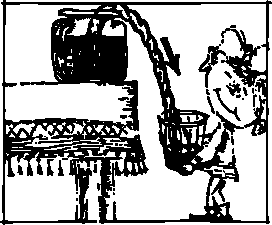
\includegraphics[width=0.6\textwidth]{figures/fig-02-05.pdf}
\caption{A siphon works on the basis of capillary action.}
\label{fig-2.5}
\end{figure}

Plants and trees have an entire system of long ducts and pores. The diameters of these ducts are less than hundredths of a millimetre. Because of this, capillary forces raise soil moisture to a considerable height and distribute water throughout the plant.

Blotting paper is a very convenient thing. You spilled some ink on a page and want to turn it over. But you’re not going to wait until the blot dries up. You take a sheet of blotting paper, dip one of its edges in the drop, and the ink swiftly runs upwards against gravity.

A typical capillary phenomenon has occurred. If you look at the blotting paper through a microscope, you can see its structure. Such a paper consists of a sparse network of paper fibres forming thin and long ducts with each other. These ducts play the role of capillary tubes.

The same kind of system of long pores or ducts formed by fibres exists in wicks. Kerosene rises through the wick of a lamp. A siphon can also be created with the aid of a wick by placing one of its ends in a glass partially filled with water, in such a way that the other end hanging over the edge is lower than the first (\figr{fig-2.5}).

In the technology of the dyeing industry, frequent use is also made of the ability of a fabric to draw in a liquid through the thin pores formed by the threads of the fabric.

We have not said anything yet about the molecular mechanism of these interesting phenomena.

The differences in the surface tension of various substances can be excellently explained by intermolecular interactions.

A drop of mercury does not spread out over the surface of glass. The reason is that the energy of interaction between the mercury atoms is greater than the energy of cohesion between the glass and mercury atoms. For the same reason, mercury does not rise in narrow capillary tubes.

It is a different matter with water. It was found that the atoms of hydrogen of the water molecules readily cohere to the atoms of oxygen in the silica of which glass mainly consists. The water-glass intermolecular forces are greater than the water-water intermolecular forces. Therefore, water spreads out into a thin film over the surface of glass and rises in glass capillary tubes.

Surface tension or, more precisely, the energy of cohe­sion (depth of the potential well in \figr{fig-2.1}) for various pairs of substances can be both measured and calculated. A discussion on how this can be done would lead us too far away from our subject.


\section{Crystals and Their Shape}

Many people think that crystals are beautiful, rarely found stones. They occur in various colours, are usually transparent and, what is most remarkable, possess a beautiful regular shape. Crystals are most often polyhedra with ideally plane sides (faces) and strictly straight edges. They please the eye with a marvellous play of colours at the faces and an amazingly regular structure.

Among them are the unassuming crystals of rock salt natural sodium chloride, i.e. common salt. They are found in nature in the form of rectangular parallelepipeds or cubes. Calcite crystals also have a simple form -- trans­parent oblique-angled parallelepipeds. Quartz crystals are much more complicated. Each little crystal has a great many faces of different shapes, intersecting in edges of different lengths.

However, a crystal is anything but a museum-piece. Crystals surround us everywhere. The solid bodies with which we build homes and make machines, the substances which we use in our daily lives almost all of them are crystals. But why do we not see this? The reason is that in nature we rarely come across bodies in the form of single individual crystals (or, as is said, monocrystals). Substances are most often found in the form of firmly linked crystalline grains of very small size, less than a thousandth of a millimetre. Such a structure can only be seen through a microscope.

Bodies consisting of tiny crystalline grains are called polycrystaltine (derived from the Creek \emph{polys} meaning ``many'').

Of course, polycrystalline  bodies must also be included among the crystals. It will then turn out that almost all the solid bodies surrounding us are crystals. Sand and granite, copper and iron, the salol sold in a drugstore and paint all these are crystals.

There are exceptions; glass and plastics do not con­sist of small crystals. Such solid-bodies are called amorphous.

Thus, studying crystals means studying almost all the bodies surrounding us. It is obvious that this is important. 

Single crystals are recognized at once by the regularity of their shapes: Plane faces and straight edges are char­acteristic properties of a crystal; the regularity of shape is undoubtedly related to the regularity of the internal structure of a crystal. If a crystal has been especially stretched in a certain direction, it means that the struc­ture of the crystal in this direction is also special in some way.

But imagine that a ball has been made by machine out of a large crystal. Will we succeed in figuring out that we have a crystal in our hands, in distinguishing this ball from a glass ball? Since the different faces of a crystal are developed to different degrees, this suggests that the physical properties of a crystal also differ in different directions. This, of course, refers to the strength of a crystal, its electrical conductivity and to many other properties. This peculiarity of a crystal is called the anisotropy of its properties. Anisotropic means different properties in different directions.

Crystals are anisotropic. On the contrary, amorphous bodies, liquids and gases are isotropic, i.e. possess iden­tical (derived from the Greek \emph{isos} meaning ``equal'') properties in different directions (derived from the Greek \emph{tropos} meaning ``turning''). The anisotropy of the proper­ ties of a crystal is precisely what permits us to find out whether or not a transparent, formless piece of matter
is a crystal.

Let us visit a mineralogical museum and closely exam­ine various monocrystalline specimens of crystals of the same substance. It is quite possible that specimens of both regular and irregular shapes are on display. Some of the crystals resemble fragments, others have one or two abnormally developed faces.

From the collection of specimens we select the ones that seem to be of perfect shape and sketch them. The drawing we obtain is shown in \figr{fig-2.6}. Quartz has again been taken as an example. As the crystals of other substances, quartz can develop a different number of faces of each ``kind'', as well as a different number of ``kinds'' of faces. Even if their similarity in appearance is not self-evident, such small crystals do resemble one another as do close relatives or, sometimes, as twins. In what does their similarity consist?

\begin{figure}[!ht]
\centering
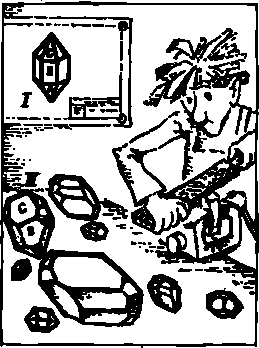
\includegraphics[width=0.6\textwidth]{figures/fig-02-06.pdf}
\caption{Different shapes of crystals.}
\label{fig-2.6}
\end{figure}

Look carefully at \figr{fig-2.6}, which illustrates a number of quartz crystals. All of them are close ``relatives'' They can be made truly similar by grinding off various faces by different amounts in such a way that they remain parallel to their initial positions. It is readily evident, for instance, that crystal $II$ can be made, in this way, entirely similar to crystal $I$. This is possible because the angles are equal between like faces, for example, be­tween faces $A$ and $B$, $B$ and $C$, etc.

It is this equality of angles that gives the crystals their ``family'' resemblance. As the faces are ground off parallel to their initial positions, the shape of the crystal is changed, but the angles between the faces are retained.

As a crystal grows, certain of its faces, due to various random factors, may be in more favourable, and others in less favourable conditions for the addition of new layers of atoms or molecules. Crystals grown under different conditions may not appreciably resemble one another, as far as their appearance is concerned, but the angles be­tween the corresponding faces of all crystals of the substance being considered are always the same. The shape (or \emph{habit}, as it is called) of a crystal is a matter of chance, but the angles between its faces (and you will understand why further on) depend upon its internal structure.

The flatness of its faces is not the only feature that distinguishes a crystal from shapeless bodies. A crystal also possesses symmetry. The meaning of this word, in the sense we are about to employ, can best be demonstrat­ed by examples.

\begin{figure}[!ht]
\centering
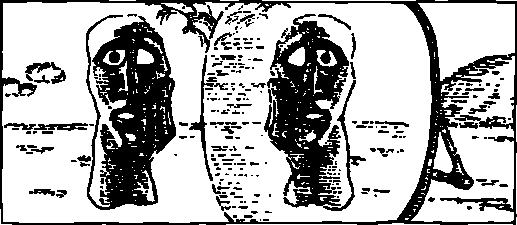
\includegraphics[width=\textwidth]{figures/fig-02-07.pdf}
\caption{Mirror symmetry.}
\label{fig-2.7}
\end{figure}


Illustrated in \figr{fig-2.7} is a statue (reminding us of the famous ones on Easter Island) standing in front of a large mirror. The reflection in the mirror is an exact copy (actually a mirror image) of the statue. The sculptor could have carved two statues and arranged them in the same manner as our statue and its reflection in the mirror.

This double sculpture is a symmetrical figure; it consists of two equal parts, one being a mirror image of the other and equal in the sense that one’s left hand is equivalent to one’s right.

Let us assume that a flat mirror is placed as in \figr{fig-2.7} Then the right-hand part of the sculpture exactly coincides with the reflection of its left-hand part. Such symmetrical arrangement would have a vertical plane of mirror symmetry passing through the centre between the two parts. The plane of symmetry is an imaginary one, but we sense it distinctly in examining a symmetrical body.

The bodies of animals have planes of symmetry; a ver­tical plane of external symmetry can be passed through a man as well. Symmetry is only approximate in the animal world, and, in general, there is no ideal symmetry in the world around us. An architector can design a house consisting of two ideally symmetrical halves. But when the house is built, no matter how well, you can always find some difference in the two symmetrical parts: one may have a crack at some place where the other has not.

The most exact symmetry is found in the world of crystals, though it is hardly ideal here either. Fissures invisible to the naked eye, scratches and other flaws always make equal faces differ slightly from one another.

The child’s toy called a pinwheel is illustrated in \figr{fig-2.8}. It is also symmetrical, but you cannot pass a plane of symmetry through it in any way. What then is symmetrical about this toy? First, let us consider its symmetrical parts. How many are there? Obviously, four. What makes their mutual arrangement regular? This, too, is simple enough. Let us turn the pinwheel counterclockwise through a right angle, i.e. one-fourth of a revolution. Now vane / has turned to the previous position of vane 2, 2 to that of vane 3, 3 to that of vane 4, and 4 to that of vane 1. The new position of the pinwheel cannot be distinguished from the previous one. We say that such a figure has an axis of symmetry or, more pre­cisely, an axis of four-fold symmetry because it coincides with itself after turning through one-fourth of a revolu­tion.

\begin{figure}[!ht]
\centering
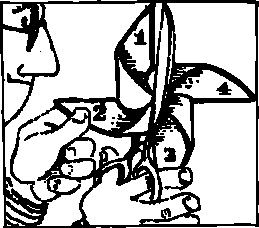
\includegraphics[width=0.6\textwidth]{figures/fig-02-08.pdf}
\caption{A pinwheel has four-fold symmetry.}
\label{fig-2.8}
\end{figure}



Thus, an axis of rotation symmetry is an imaginary straight line about which a body, when turned through a unit fraction of a revolution, is in a position that can­ not be distinguished from its initial position. The order of rotation symmetry (four-fold in our case) indicates that such coincidence occurs after turning the body one-fourth of a revolution. Consequently, after four such turning motions we return to the initial position.

Do we find symmetry of all kinds in the crystal king­dom? Investigations have shown that we do not. In fact, the only axes of rotation symmetry found in crystals are the two-, three-, four- and six-fold ones. This is no mere chance. Crystallographers have shown that it is related with the internal structure of crystals. Therefore, the number of different kinds or, as we say, classes of crystal symmetry is relatively small -- only 32.

\section{Structure of Crystals}

Why is the regular shape of a crystal so beautiful? Its faces, so smooth and shining, look as though they were polished by a skilled lapidary. Different parts of the crystal repeat one another, forming a handsome sym­metrical figure. This exceptional regularity of crystals has been known since time immemorial. But the con­cepts of the ancient scholars on the nature of crystals differed only slightly from the tales and legends made up by poets whose imagination was fascinated by the beauty and elegance of crystals. It was believed that rock crystal is formed of ice, and diamonds of rock crystal. Many wonderous properties were attributed to crystals; they were thought to heal diseases, protect one against poisons, have an influence on one’s fate and many others.

\begin{figure}[!ht]
\centering
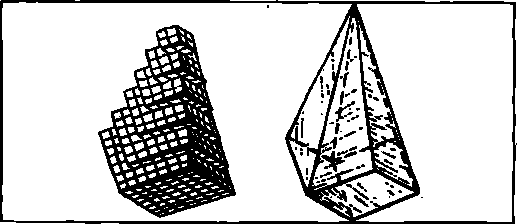
\includegraphics[width=\textwidth]{figures/fig-02-09.pdf}
\caption{The structure of crystals made up of tiny ``building blocks''.}
\label{fig-2.9}
\end{figure}



The first scientific views on the nature of crystals appeared only in the $17^{\textrm{th}}$ and $18^{\textrm{th}}$ centuries. An idea of these conceptions is given by \figr{fig-2.9}, which was reproduced from \emph{Traite de Mineralogie}, written by the French abbe, Rene Just Ha\"uy, near the end of the 18th century. 

According to its author, crystals are made up of tiny ``building blocks'', fitting tightly to one another. This conclusion is one that is naturally arrived at. Let us break up a crystal of Iceland spar (calcite, or calcium carbonate) with a sharp blow of a hammer. It flies apart into pieces of various sizes. Examining them carefully, we find that the pieces are of regular shape, quite similar to that of the large crystal, their ``parent'' Evidently, reasoned Ha\"uy, if we continue to break up the pieces into smaller and smaller ones, we will finally reach the smallest building block, invisible to the naked eye, which is a crystal of the given substance. These ultimate blocks are so small that steps formed by them, comprising the faces of the large crystal, seem to us to be immaculately smooth. Well, and what is this final building block like? The scientists of that day could not answer this question.

The ``building block'' theory of crystal structure was of great benefit to science. It explained the origin of the straight edges and flat faces of a crystal. As a crystal grows, new building blocks attach themselves to those of the crystal, and a face grows like the wall of a house built by the hands of bricklayers.

Hence, the question concerning the reason for the regularity and beauty of the shapes of crystals has been answered a long time ago. The reason for this phenom­enon is their internal regularity. This regularity consists in the endless repetition of one and the same ele­mentary parts.

Imagine a park fence made of rods of different lengths and distributed helter-skelter. An ugly scene. A good fence is constructed from identical rods distributed in a regular sequence at equal distances from each other. We find such a self-repeating pattern on wallpaper. Here an element of a drawing, say, a girl playing with a ball, is repeated not only in one direction, as in a park fence, but so that it fills a plane.

\begin{figure}[!ht]
\centering
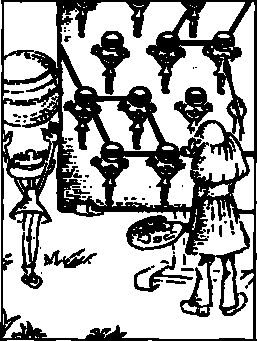
\includegraphics[width=0.6\textwidth]{figures/fig-02-10.pdf}
\caption{Finding a ``unit cell'' in a wallpaper pattern.}
\label{fig-2.10}
\end{figure}

But what relationship do a park fence and wallpaper have to a crystal? A most direct one. A park fence consists of links repeating along a line, wallpaper of pat­terns repeating in a plane, and a crystal of groups of atoms repeating in space. One therefore says that the atoms of a crystal form a space (or crystal) lattice.

There are certain details concerning a three-dimensional, or space, lattice that we must now discuss. To sim­plify the work of the illustrator, we shall explain all that is required, using wallpaper as an example, rather than asking him to construct complicated drawings of three-dimensional figures.

Separated out in \figr{fig-2.10} is the smallest piece that can be transferred or shifted to obtain the whole pattern of the wallpaper. To separate out such a piece, we draw two straight lines from any point of the drawing, for instance, the centre of the beach ball, connecting it to the same points of the two adjacent balls. As can be seen in our drawing, we can use these two lines to construct a parallelogram. By shifting or transferring this parallelogram along the directions of the two initial basic lines over distances equal to its sides, we can obtain the whole wallpaper pattern. This smallest repeated portion, commonly called a unit cell, can be selected in various ways. It is evident from \figr{fig-2.10} that several different parallelograms could be selected, each containing one drawing. We emphasize that in the given case it makes no difference to us whether the picture inside the cell is a whole one or it is divided up by the lines bounding the cell.

It would be a mistake to suppose that after drawing the repeating picture, called the motif, for the wallpaper the artist can always consider his job to be finished. This would be true if the only way to make a pattern for wallpaper was to add to the given portion another identi­cal portion, shifted parallel to the first along the two initial basic lines.

\begin{figure}[!ht]
\centering
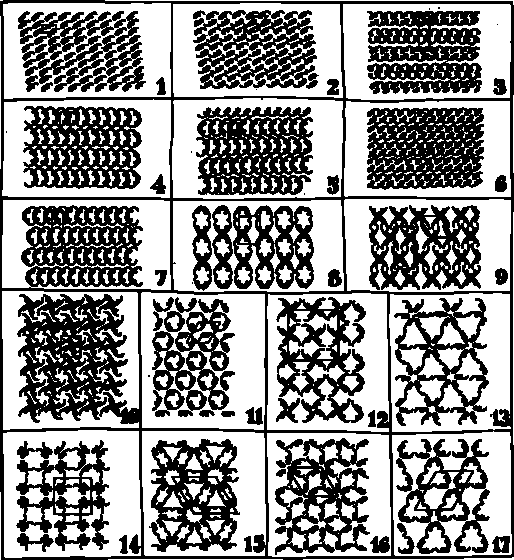
\includegraphics[width=\textwidth]{figures/fig-02-11.pdf}
\caption{Seventeen possible ways to fill the wallpaper design, that is filling the plane.}
\label{fig-2.11}
\end{figure}


In addition to this simplest method, however, there are sixteen more ways to fill in the wallpaper design with an orderly repeated drawing, or motif, i.e. seventeen types of mutual arrangement of drawings on a plane. They are illustrated in \figr{fig-2.11}. Here a simpler repeating motif has been selected, but, like the one in \figr{fig-2.10}, it has no symmetry in itself. The patterns composed of this motif are symmetrical and the difference in the patterns is due to the difference in the symmetrical arrangements of the motifs.

We see, for example, that in the first three cases the pattern has no plane of mirror symmetry: you cannot position vertical mirror so that one part of the pattern is a mirror reflection of another part. Cases 4 and 5, on the contrary, have planes of symmetry. Two mutually perpendicular mirrors can be set up in cases 8 and 9.

Case 10 has an axis of four-fold rotation symmetry, per­pendicular to the plane of the drawing. In case 11, the axis is of three-fold symmetry, and in cases 13 and 15, of six-fold rotation symmetry.

Planes and axes of symmetry are found on our drawings in parallel series or families, rather than singly. If you have found one point through which you can pass an axis (or plane) of symmetry, you can readily find the adjacent point and consecutive points, all spaced at the same distance from one another, through which the same kind of axes (or planes) of symmetry can be passed.


\begin{figure}[!ht]
\centering
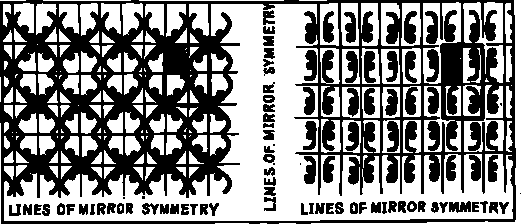
\includegraphics[width=\textwidth]{figures/fig-02-12.pdf}
\caption{Two illustrations for Case 8 type of pattern.}
\label{fig-2.12}
\end{figure}

The seventeen types of symmetry of a plane pattern do not, of course, exhaust all of the great variety of patterns that can be composed from a single motif. The artist must specify one more condition: how the motif is to be positioned with respect to the boundary lines of the cell. \figr{fig-2.12} illustrates two wallpaper pat­terns with the same initial motif which is differently positioned in each pattern with respect to the lines rep­ resenting the vertical mirrors (in a plane pattern they are simply lines of symmetry). Both patterns come under case 8 in \figr{fig-2.11}.

Each body, including crystals, consists of atoms. Simple substances, or elements, consist of atoms of a single kind. Complex substances, or compounds, con­sist of atoms of two or several kinds. Assume that in some superpowerful microscope we could examine the surface of a crystal of common salt and see the centres of the atoms. \figr{fig-2.13} shows how we would see the atoms arranged along a face of the crystal like a wallpaper pattern. You can readily understand now how a crystal is constructed. We could say that a crystal resembles ``three-dimensional wallpaper''. A crystal is composed by joining three-dimensional unit cells tightly together instead of plane cells as for wallpaper patterns. These three-dimensional unit cells are the building blocks of which the crystals are built.

\begin{figure}[!ht]
\centering
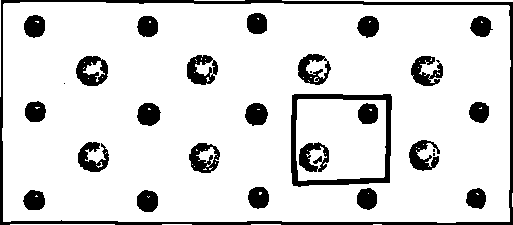
\includegraphics[width=\textwidth]{figures/fig-02-13.pdf}
\caption{A crystal as a ``three-dimensional wallpaper''.}
\label{fig-2.13}
\end{figure}


How many different ways exist for building up three- dimensional wallpaper patterns from these elementary pieces? This complex mathematical problem was solved at the turn of the century by the founder of structural crystallography Yevgraf Stepanovich Fedorov (1853- 1919). This eminent Russian scientist established the fact that there can be only 230 different ways to build up a crystal or, as they say today, 230 Fedorov groups.

All that is known today about the internal structure of crystals was obtained by $X$-ray structure analysis, which we shall describe in some detail in the fourth book.

Simple crystals exist, made up of atoms of a single kind. Diamond, for example, is of pure carbon. Crystals of common salt consist of ions (electrically charged atoms) of two kinds: sodium and chlorine. More complex crystals may be made up of molecules which, in their turn, consist of atoms of many kinds.

We can always single out in a crystal the smallest repeating groups of atoms (or single atoms, in the simplest case). Such a group is called the unit cell. \label{unit-cell-def}

The dimensions of unit cells may vary in wide ranges. The shortest distances are found between the adjacent lattice points (corners of the unit cell) of the simplest crystals, consisting of atoms of a single kind. The maximum distances are found in complex protein crystals. These distances, called lattice constants, range from 2 or 3 angstroms to several hundred angstroms (hund­redths of one-millionth of a centimetre).

There are a great variety of crystal lattices. The prop­erties common to all crystals are due to their lattice structure. To begin with, we can readily understand that the ideally flat faces of a crystal are the planes passing through the lattice points at which atoms are located. But any number of lattice planes can be passed in the most diverse directions. Which of these planes bound the grown crystals, i.e. become its faces?

Let us turn our attention, first of all, to the following circumstance: various lattice planes and lines are not filled equally densely with lattice points. Experiments show that a crystal is faceted by the planes that are most densely studded with lattice points and that these planes intersect at edges which are also most densely occupied by lattice points.

\begin{figure}[!ht]
\centering
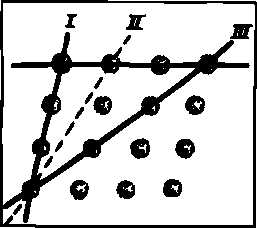
\includegraphics[width=0.6\textwidth]{figures/fig-02-14.pdf}
\caption{A view of a crystal perpendicular to a face.}
\label{fig-2.14}
\end{figure}

A view of a crystal lattice perpendicular to a face is shown in \figr{fig-2.14}. Shown also are the traces of lattice planes perpendicular to the drawing. It should be clear from what has been said that faces on the crystal parallel to planes $I$ and $III$ are apt to develop. No faces will be developed parallel to plane $II$ which is so sparsely dotted with lattice points (and atoms).

The structures of many hundreds of crystals are known today. We shall discuss the structures of the simplest crys­tals, first of all, those built up of atoms of a single kind.

Three types of lattices are most common. They are shown in \figr{fig-2.15}. The centres of the atoms are repre­sented by points; the lines joining the points do not have any actual meaning. They have been drawn merely to make the nature of the spatial distribution of the atoms clearer to the reader.

\figr{fig-2.15}~\textcolor{black!70}{(a)} and \textcolor{black!70}{(b)} depict cubic lattices. In order to visualize these lattices more clearly, imagine that you have arranged building blocks in the simplest manner -- edge to edge and face to face. If you now conceptually place points at the vertices and centres of the cubes, the cubic lattice depicted in \figr{fig-2.15}~\textcolor{black!70}{(a)} appears. Such a structure is called body-centred cubic. If points are placed at the vertices of the cubes and at the centres of their faces, the cubic lattice depicted in \figr{fig-2.15}~\textcolor{black!70}{(b)} appears. It is called face-centred cubic.


\begin{figure}[!ht]
\centering
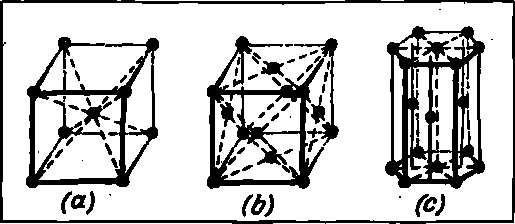
\includegraphics[width=\textwidth]{figures/fig-02-15.pdf}
\caption{Three types of common lattices.}
\label{fig-2.15}
\end{figure}

The third lattice (\figr{fig-2.15}~\textcolor{black!70}{(c)}) is called close-packed hexagonal (i.e. having six angles). In order to understand the origin of this term and more clearly visualize the distribution of the atoms in this lattice, let us take some billiard balls and start packing them as closely as pos­sible. First of all, let us form a close layer -- it looks like billiard balls which have been gathered in by a rack before the beginning of a game (\figr{fig-2.16}). Note that the ball in the middle of the triangle is in contact with six neighbours, and these six neighbours form a hexagon.

We continue the packing by laying one layer upon ano­ther. If we place the balls of the second layer directly above the balls of the first, such a packing would not be close. Trying to distribute the greatest number of balls in a definite volume, we should place the balls of the second layer in the holes formed by the first, the balls of the third layer in the holes of the second, etc. In a close-packed hexagonal lattice, the balls of the third layer are placed in such a way that their centres lie directly above those of the balls of the first.

\begin{figure}[!ht]
\centering
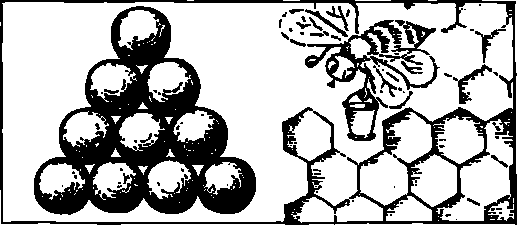
\includegraphics[width=\textwidth]{figures/fig-02-16.pdf}
\caption{Two examples of hexagonal lattice: a rack of billiard balls, the structure of a beehive.}
\label{fig-2.16}
\end{figure}

The centres of the atoms in a close-packed hexagonal lattice are distributed just like those of the balls which
are closely packed in the manner described.

A great many elements crystallize in the lattices of the
three types described above:

\begin{center}
\begin{small}
\begin{tabular}{p{5.25cm}p{4cm}}
\toprule
Close-packed hexagonal lattice & \ce{Be}, \ce{Co}, \ce{Hf}, \ce{Ti}, \ce{Zn}, \ce{Zr} \\
Face-centred cubic & \ce{Al}, \ce{Cu}, \ce{Co}, \ce{Fe}, \ce{Au}, \ce{Ge}, \ce{Ni}, \ce{Ti} \\
Body-centred cubic & \ce{Cr}, \ce{Fe}, \ce{Li}, \ce{Mo}, \ce{Ta}, \ce{Ti}, \ce{U}, \ce{V}\\
\bottomrule
\end{tabular}
\end{small}
\end{center}

We shall mention only a few of the other structures. The structure of diamond is depicted in \figr{fig-2.17}. What is characteristic of this structure is that a carbon atom in diamond has four immediate neighbours. Let us compare this number with the corresponding numbers for the three most common structures just described. As is evident from the figures, each atom has 12 immediate neighbours in a close-packed hexagonal lattice, the atoms forming a face-centred cubic lattice have just as many neighbours, and each atom has eight neighbours in a body-centred lattice.

\begin{figure}[!ht]
\centering
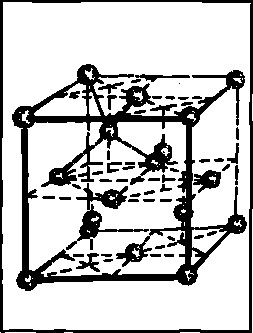
\includegraphics[width=0.5\textwidth]{figures/fig-02-17.pdf}
\caption{Crystal structure of a diamond.}
\label{fig-2.17}
\end{figure}

We shall say a few words about graphite, whose struc­ture is shown in \figr{fig-2.18}. This structure has a striking peculiarity. Graphite consists of layers of atoms, where atoms of a single layer are more firmly bound to each other than atoms of neighbouring layers. This is related to the values of the interatomic distances: the distance between neighbours in a single layer is 2.5 times as small as the shortest distance between layers.

\begin{figure}[!ht]
\centering
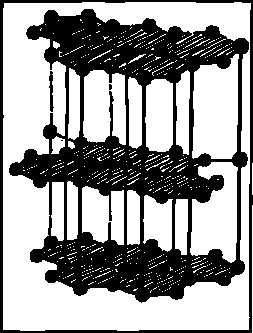
\includegraphics[width=0.5\textwidth]{figures/fig-02-18.pdf}
\caption{Crystal structure of graphite.}
\label{fig-2.18}
\end{figure}

The presence of weakly bound atomic layers makes it easy for graphite crystals to break up along these layers. This is why solid graphite can serve as a lubricant in those cases when it is impossible to apply lubricating oil -- for example, at very low or very high temperatures. Graphite is a solid lubricant.

Friction between two bodies reduces, roughly speaking, to the fact that microscopic protuberances of one body fall in hollows of the other. The force required for breaking up a microscopic graphite crystal is much smaller than the frictional forces; therefore, a graphite lubrication considerably facilitates the sliding of one body along another.

There is an endless variety in the structures of crystals of chemical compounds. The structures of rock salt and carbon dioxide depicted in Figures 2.19 and 2.20 can serve as extreme examples.

\begin{figure}[!ht]
\centering
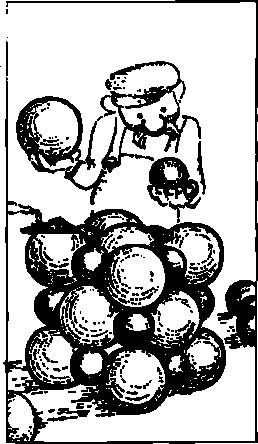
\includegraphics[width=0.5\textwidth]{figures/fig-02-19.pdf}
\caption{Crystals of rock salt.}
\label{fig-2.19}
\end{figure}

Crystals of rock salt (\figr{fig-2.19}) consist of atoms of sodium (small dark balls) and chlorine (large light balls) alternating along the axes of a cube. Each sodium atom has six equidistant neighbours of the other kind. The same is also true of chlorine. But where are the molecules of sodium chloride? There are none; not only are groups of single atoms of sodium and single atoms of chlorine absent from salt crystals, but in general, no group of atoms whatsoever can be distinguished from the others by their proximity.

The chemical formula of NaCl does not give us any
grounds for saying that ``this substance is built up out of molecules of \ce{NaCl}''. The chemical formula merely indicates that the substance is constructed from the same number of atoms of sodium and chlorine.

\begin{figure}[!ht]
\centering
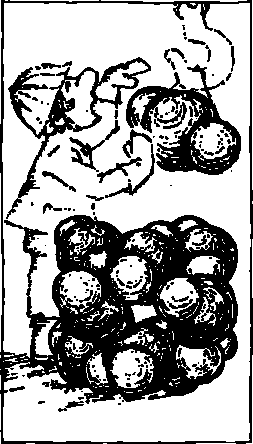
\includegraphics[width=0.5\textwidth]{figures/fig-02-20.pdf}
\caption{Crystal structure of carbon dioxide \ce{CO2}.}
\label{fig-2.20}
\end{figure}

The question of the existence of molecules in a substance is decided by its structure. If no groups of close atoms can be distinguished in it, there are no molecules.


A crystal of carbon dioxide, \ce{CO2} (the dry ice which lies in cartons of ice cream), is an example of a molecular crystal \figr{fig-2.20}.

The centres of the oxygen and carbon atoms of a molecule of \ce{CO2} are situated along a straight line (see \figr{fig-2.2}­). The distance \ce{C-O} is equal to \SI{1.3}{\angstrom}, and the distance between oxygen atoms of neighbouring molecules is about \SI{3}{\angstrom}. It is obvious that under such conditions we immediately ``recognize'' a molecule in a crystal.

Molecular crystals are close packings of molecules. In order to see this, we must outline the contours of the molecules. This is precisely what has been done in \figr{fig-2.20}.


\begin{figure}[!ht]
\centering
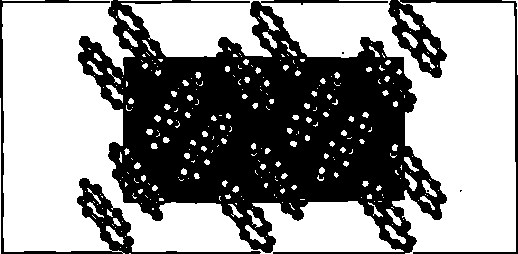
\includegraphics[width=\textwidth]{figures/fig-02-21.pdf}
\caption{Crystal structure of an organic substance.}
\label{fig-2.21}
\end{figure}

All organic substances consist of molecular crystals. Organic molecules frequently consist of many tens and even hundreds of atoms (those made up of tens of thousands of atoms are to be discussed in a separate chapter). It is impossible to properly depict their packing arrangements graphically. For this reason, you may find drawings similar to \figr{fig-2.21} in books in this field. The mole­cules of this organic substance are built up of carbon atoms. The bars between the atoms represent the valence bonds. The molecules seem to be suspended in air. But do not believe what you see here. They have been drawn thus to give you an idea of how the molecules are arranged in a crystal. For the sake of simplicity, the illustrator did not show the hydrogen atoms joined to the outer atoms of carbon (as a matter of fact, chemists frequently make their similar omissions). He did not even consider it necessary to outline the molecule, imparting a definite shape to it. If he had, we would see that the principle of molecular packing, with the ``key fitting the lock'', is just as valid in this case as in other similar ones.



\section{Polycrystalline Substances}

We have already mentioned the fact that amorphous bodies are rare in the world of solids. Most of the objects surrounding us consist of tiny crystalline grains, about a thousandth of a millimetre in size.

Investigators discovered the granular structure of met­als in the $19^{\textrm{th}}$ century with the aid of ordinary optical microscopes. All that was required was an arrangement enabling the specimens to be observed in reflected instead of transmitted light. Up-to-date metallurgical microscopes operate on this same principle.

The image seen in such a microscope may be like that shown in \figr{fig-2.22}. The grain boundaries are usually quite distinct. As a rule, impurities accumulate at the boundaries.

\begin{figure}[!ht]
\centering
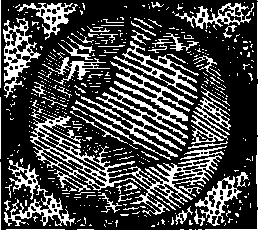
\includegraphics[width=0.6\textwidth]{figures/fig-02-22.pdf}
\caption{Crystal structure of a metal.}
\label{fig-2.22}
\end{figure}

The properties of materials depend to an exceptionally large degree on the size of the grains, their orientation and what is happening at their boundaries. For this reason, physicists have devoted much research to the study of polycrystalline substances. By means of $X$-ray structure analysis, about which we have already promised to tell our readers, they found that each grain is a small crystal. We repeat our promise.

All treatment of a metal affects its grains. Suppose we have a piece of cast metal. Its grains are in disorder and their size is quite large. Then we make wire of the piece of metal by drawing it through a die. What happens to the crystalline grains in this plastic working operation? Investigations have shown that the change in shape of a solid in drawing wire or in some other plastic working technique breaks up the crystalline grains. At the same time, a certain element of order is produced in the arrange­ment of these grains by the action of the mechanical forces. But what possible kind of order can there be here? The fragments of the grains are absolutely shapeless.

This is true: the fragments may be of any random shape, but a fragment of a crystal is still a crystal and the atoms in its lattice are packed as regularly as in any well-faceted crystal. Hence, we can indicate in each fragment how its unit cells are oriented. Prior to plastic working, the cells are strictly ordered only within each separate grain; there is, as a rule, no total order. After the metal is worked, the grains align themselves so that a certain general order becomes evident in their cells. This is called \emph{texture}. For example, the diagonals of the cells in all the grains become oriented approximately parallel to the direction in which the metal is worked.

\begin{figure}[!ht]
\centering
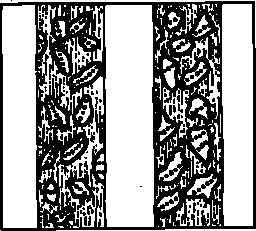
\includegraphics[width=0.6\textwidth]{figures/fig-02-23.pdf}
\caption{\emph{Texture} in a crystal.}
\label{fig-2.23}
\end{figure}

Texture is illustrated in \figr{fig-2.23} (at the right) by the example of certain definite, indicated planes in the grains. These planes are most densely filled with atoms and are shown by rows of dots. The illustration at the left shows the grains of the metal before being worked.

The various kinds of plastic working operations (roll­ing, forging, and wire-drawing) produce textures of different types. In some operations, the grains turn so that the diagonals of their unit cells are aligned along the direc­tion of working, while in others the edges of the cells are aligned, etc. The more advanced the rolling or wire­ drawing technique, the more perfect the texture of the crystalline grains of metal. Texture has a striking effect on the mechanical properties of metal articles. A study of the arrangement and size of the crystalline grains in metals led to an understanding of the fundamental prin­ciples involved in the plastic working of metals. This, in turn, led to the improvements of the techniques em­ployed.

Another important kind of metal treatment, anneal­ing, is also associated with the rearrangement of the metal grains. If rolled or drawn metal is heated to a suffi­ciently high temperature, new crystals are formed, which grow at the expense of the old ones. Annealing gradually destroys the texture; the new crystals are arranged dis­orderly. As the temperature is raised (or the metal is held longer at the annealing temperature), new grains grow and the old ones disappear. The grains can grow to a size visible to the naked eye. Annealing drastically alters the properties of a metal. It becomes more ductile and softer. This occurs because the grains become coarser and the texture disappears.


%\newpage
%\begin{center}
%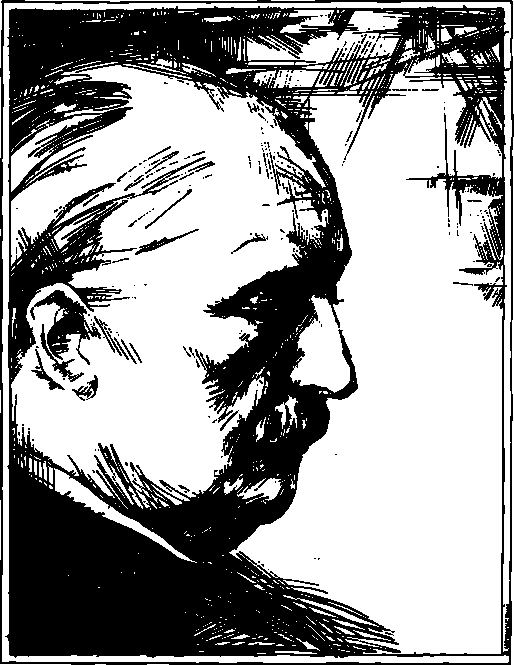
\includegraphics[width=\textwidth]{figures/helmholtz.pdf}
%\end{center}
%{\small \textbf{Hermann Helmholtz (1821-1894)} -- a famous Herman scientist. Helm­holtz worked in hie fields of physics, mathematics and physiology with great success. He was the first (1847) to give a mathematical interpretation of the law of conservation of energy emphasizing the universal character of this law. Helmholtz obtained outstanding \textcolor{red}{\textbf{incomplete}}}
%
%




